\begin{figure*}[htb]
	\center
	\begin{subfigure}[b]{0.49\textwidth}
		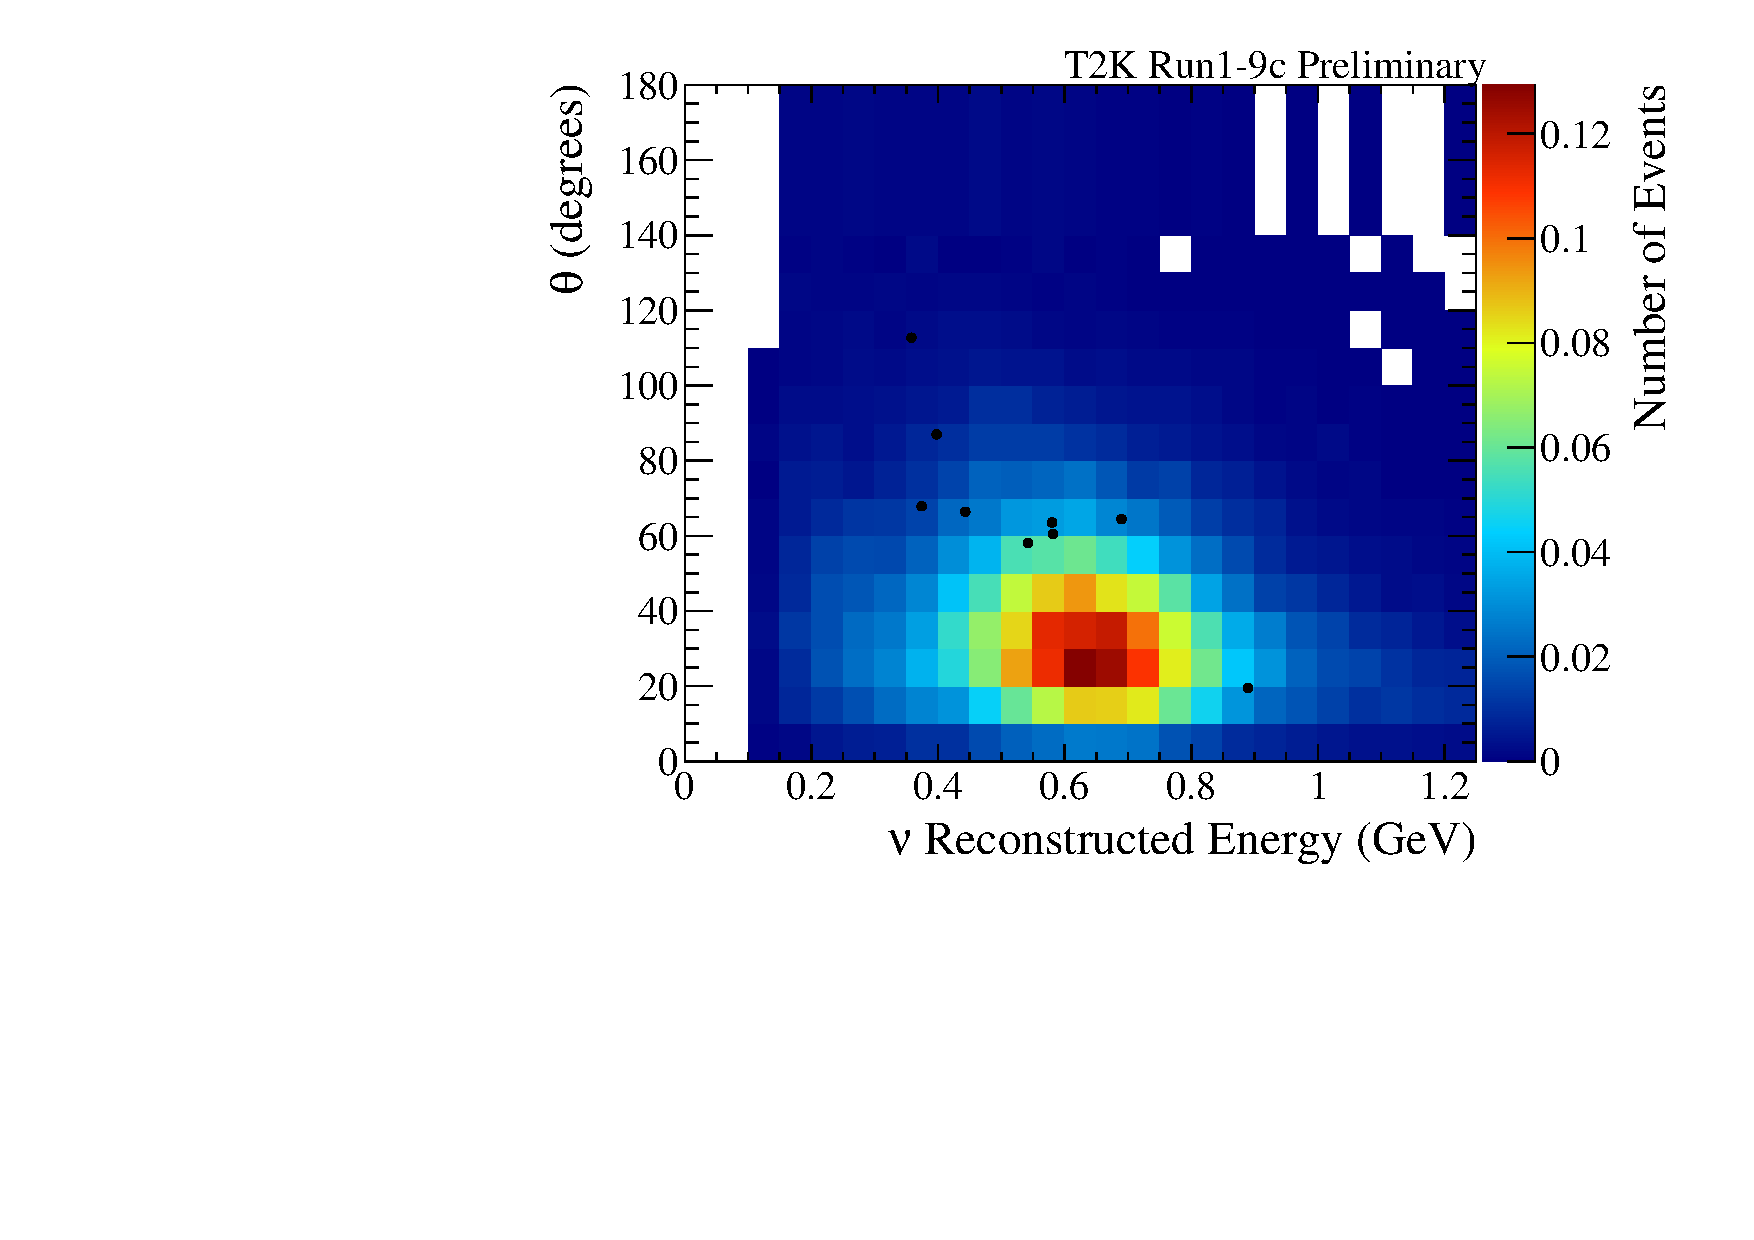
\includegraphics[width=0.9\textwidth]{spectra/components/spectrum_AsmovA_RHC1Re_NumuBarToNueBar}
		\caption{$\numub \rightarrow \nueb$}
	\end{subfigure}
	\begin{subfigure}[b]{0.49\textwidth}
		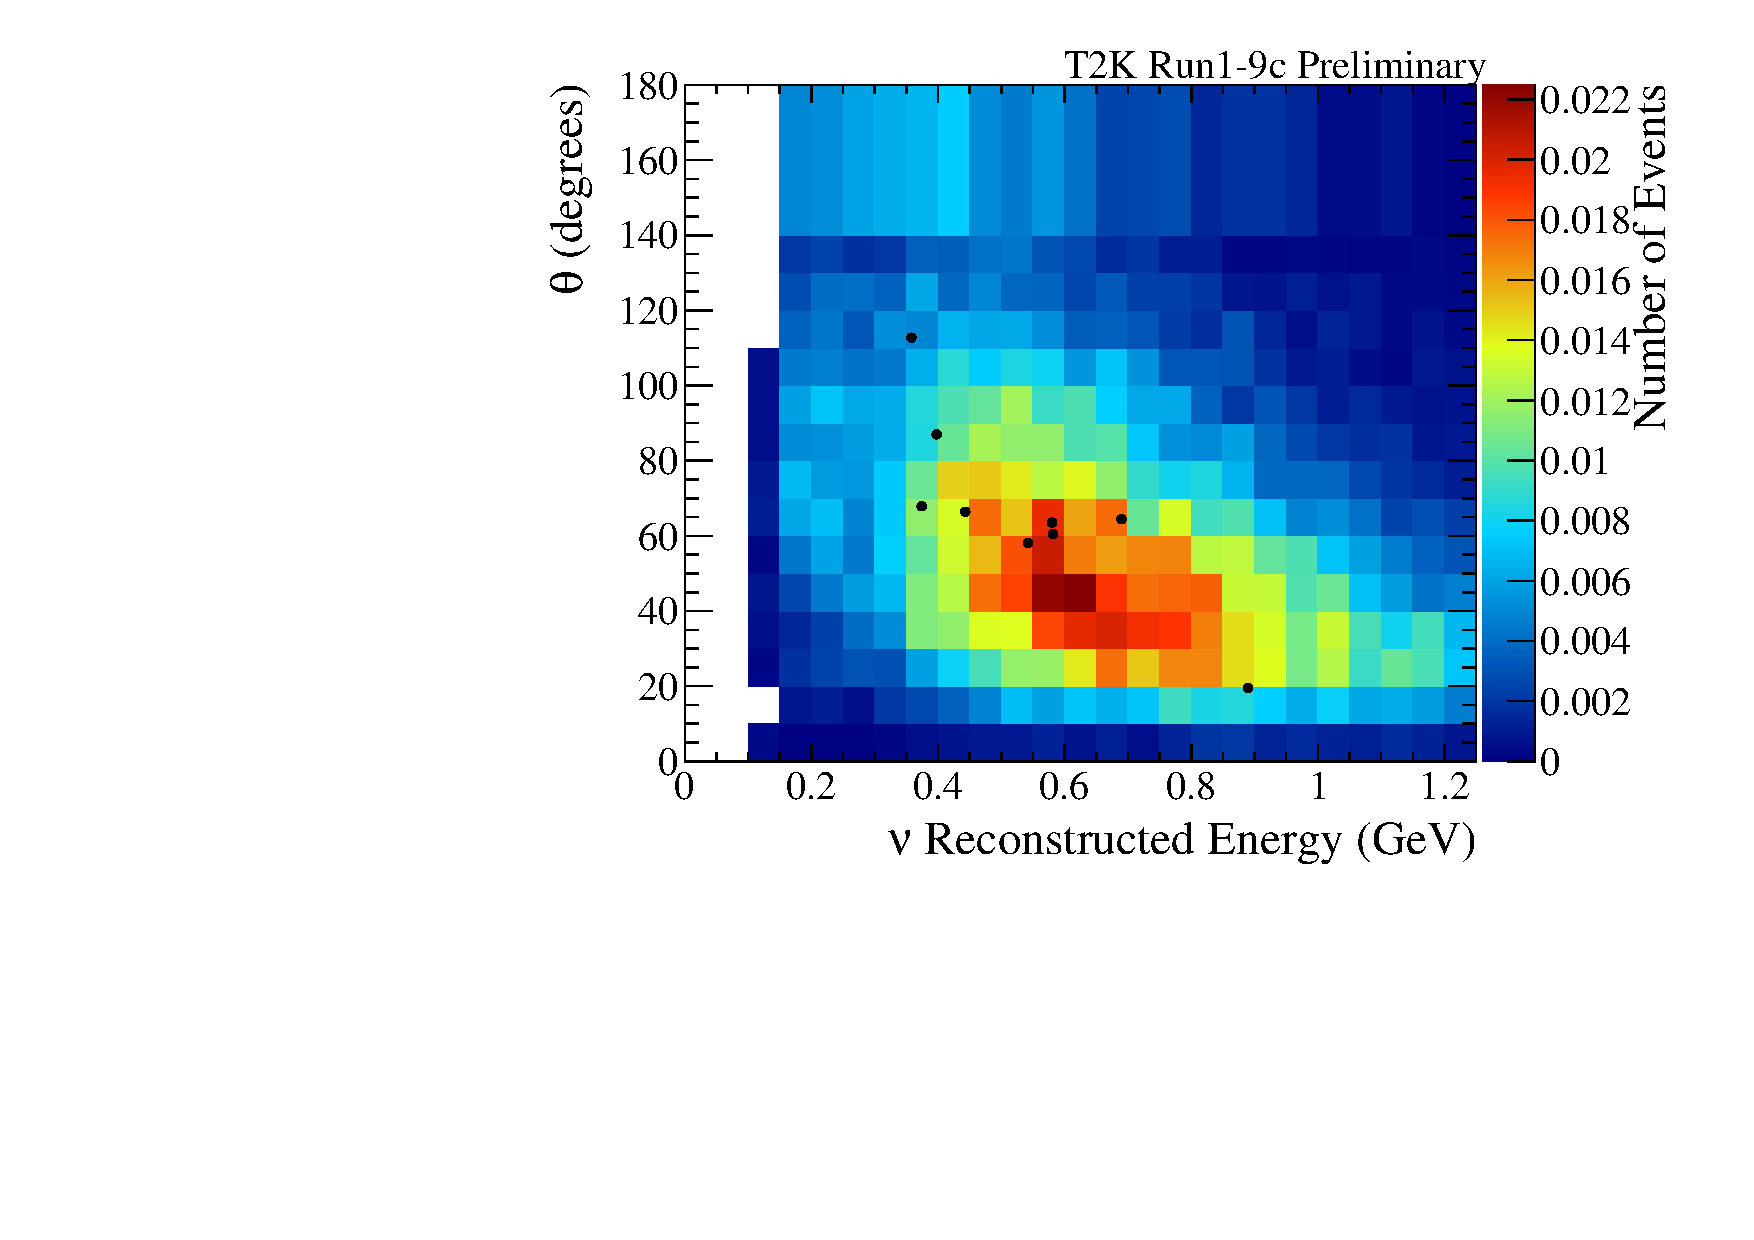
\includegraphics[width=0.9\textwidth]{spectra/components/spectrum_AsmovA_RHC1Re_NumuToNue}
		\caption{$\numu \rightarrow \nue$}
	\end{subfigure}
	\begin{subfigure}[b]{0.49\textwidth}
		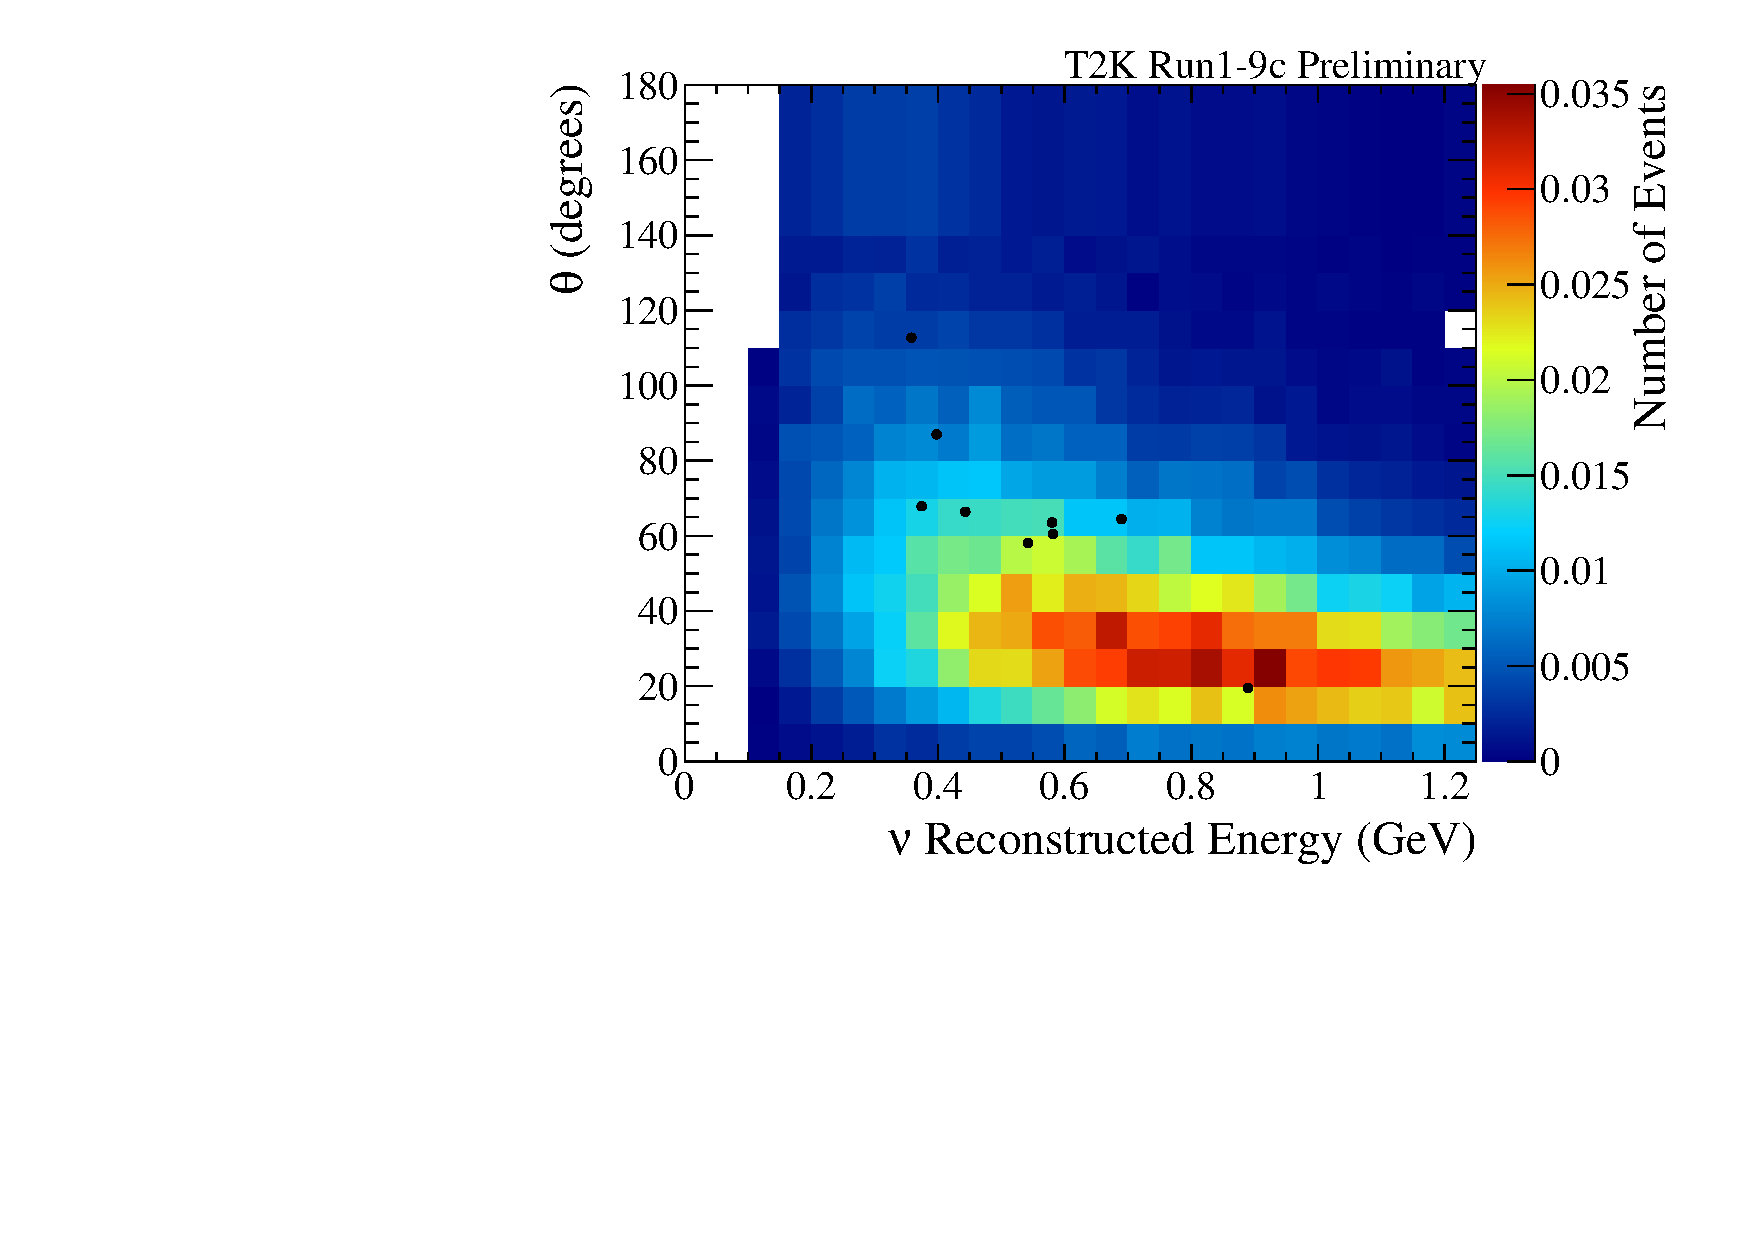
\includegraphics[width=0.9\textwidth]{spectra/components/spectrum_AsmovA_RHC1Re_NueBeam}
		\caption{Intrinsic $\nue$ + Intrinsic $\nueb$}
	\end{subfigure}
	\caption {
		Predicted Asimov A Electron-like antineutrino mode spectra broken down by component. The distributions correspond to the statistics collected in the full \RunPeriod data set. The spectra are generated with the oscillation parameters corresponding to the Asimov data set A shown in \cref{tab:osc_params_joint_asimovA}.
	}
	\label{fig:asimova_spectra_components}
\end{figure*}
\clearpage